\documentclass[12pt]{article}

\usepackage[portuguese]{babel}
\usepackage{graphicx}
\usepackage[section]{placeins}
\usepackage{float}
\usepackage{url}
\usepackage{hyperref}

\graphicspath{ {figures} }

\author{João Vitor Maia Neves Cordeiro}
\title{Relatório técnico: Análise do preço da gasolina comum entre Minas Gerais e Paraná}
\date{\today}

\begin{document}

\maketitle

\tableofcontents

\section{Introdução}

Esse relatório é a recapitulação de um trabalho realizado ao longo do semestre para a disciplina INE5405, ministrada pelo Prof. José Francisco D. de G. C. Fletes, apresentado como método de avaliação para a unidade 1 da disciplina. O trabalho consistiu de uma coleta, normalização, análise e interpretação dos dados coletados através do site da ANP sobre a precificação da gasolina comum em postos dos estados Minas Gerais e Paraná.

\section{Objeto}

\subsection{Tema}

Como já dito na seção acima, o trabalho foi realizado em cima de dados coletados no site da ANP, que podem ser encontrados neste \href{https://preco.anp.gov.br/include/Resumo_Por_Estado_Index.asp}{link}, os dados estão disponíveis para consulta pública. Foram coletados os dados para os estamos Minas Gerais e Paraná, apenas na gasolina comum.

\subsection{Delimitação do tema}

As análises foram feitas a partir de uma normalização inicial dos dados, para padronizar as planilhas coletadas em um formato mais trabalhável e de mais fácil leitura. Depois dessa normalização foi possível trabalhar tanto com dados agrupados quanto não agrupados, flexibilizando as análises e métricas possíveis de serem obtidas sobre o conjunto de dados estudado.

\subsection{Problema}

Preços de combustível utilizados em métodos de transporte cotidiano são de grande importância para a população em geral, pois além do impacto direto (transporte para o trabalho, viagens de carro e outros) existe também um impacto indireto, como o custo geral de qualquer produto que precise ser transportado até o local de venda, o custo de tarifas de transporte público e até o custo de produtos que normalmente não associamos a logística de transporte. Por isso, é necessário que sejam estudados e investigados valores discrepantes dentro de um estado, município ou bairro.

\subsection{Hipótese}

Queremos verificar se o preço do combustível possui alguma relação com a origem de sua bandeira, isto é, se por ser de uma bandeira nacional um combustível é mais caro ou mais barato do que em uma bandeira internacional, além de considerarmos também bandeiras brancas (postos que não possuem contrato).

\section{Objetivos}

Separar faixas de preço normalizadas em cada estado, aplicando técnicas para reduzir a discrepância entre dados dentro de um determinado estado e poder analisar o melhor custo-benefício para o consumidor em cada local.

\subsection{Objetivos específicos}

\section{Justificativa}

A partir do problema levantado em 2.3, pretende-se por meio da aplicações de técnicas de análises estatísticas produzir uma interpretação melhor do ponto de vista do consumidor sobre os dados coletados, auxiliando a população geral na hora de decidir em quais postos abastecer e quais bandeiras procurar.

\section{Metodologia}

\subsection{Método de abordagem}

\begin{enumerate}
    \item Primeira etapa: coleta de dados

    Utilizando a base de dados fornecida pelo site da ANP, será feita a análise sobre dados agrupados ou não, para que se possa identificar possíveis discrepâncias e taxas de maior frequência.

    \item Segunda etapa: análise descritiva dos dados
    
    Já com os dados normalizados, iremos buscar métricas estatísticas descritivas como moda, desvio padrão, variância e outras.

    \item Terceira etapa: análise exploratória dos dados
    
    Nessa parte será realizada a análise de valores discrepantes, principalmente classificados por bandeira, encontrados em etapas anteriores.
\end{enumerate}

\subsection{Técnicas de pesquisa}

\begin{enumerate}
    \item Primeira etapa: coleta de dados

    Nessa etapa usamos histogramas para visualizar as classes de frequência, modelo visual que facilita a visualização de dados agrupados, esse trabalho foi feito com o auxilio do software Excel em uma planilha de dados. 

    \item Segunda etapa: análise descritiva dos dados
    
    Já na segunda etapa utilizamos fórmulas matemáticas presentes nas referências bibliográficas da disciplina, novamente o software Excel foi utilizado para aplicar essas fórmulas no conjunto de dados e obter resultados mais precisos e menos propícios a erros de cálculo, isso foi feito já que o volume do conjunto de dados era bem significativo

    \item Terceira etapa: análise exploratória dos dados
    
    Na última etapa do trabalho, foram utilizados Box-Plots em conjunto com a regra dos quartis de Montgomery para explicitar a existência ou não de outliers e outros valores discrepantes, a afim de entregar uma análise completa do problema.
\end{enumerate}

\section{Apresentação e análise dos resultados}

\begin{figure}[H]
    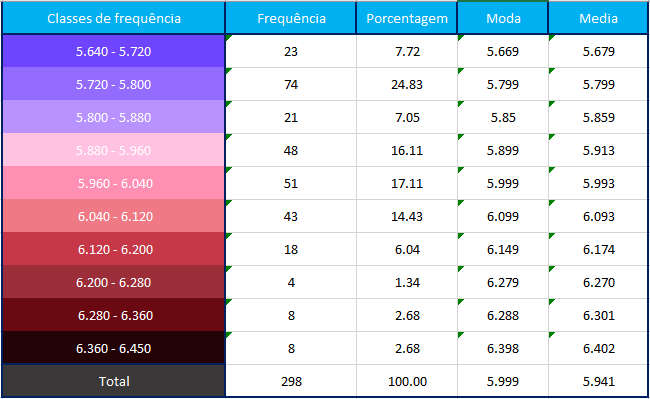
\includegraphics[width=\linewidth]{frequencias_mg.png}
    \caption{Tabela de frequências para os dados de Minas Gerais.}
\end{figure}

\begin{figure}[H]
    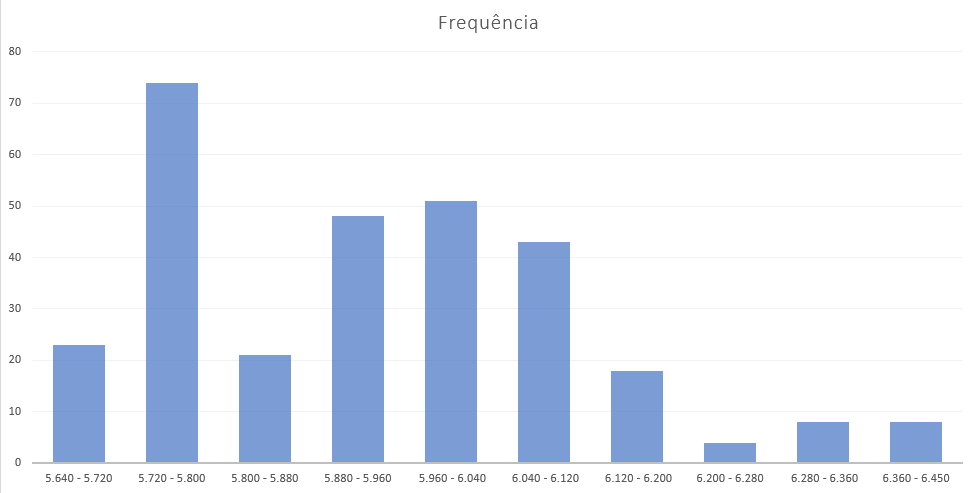
\includegraphics[width=\linewidth]{histograma_mg.png}
    \caption{Histograma das frequências para os dados de Minas Gerais.}
\end{figure}

\begin{figure}[H]
    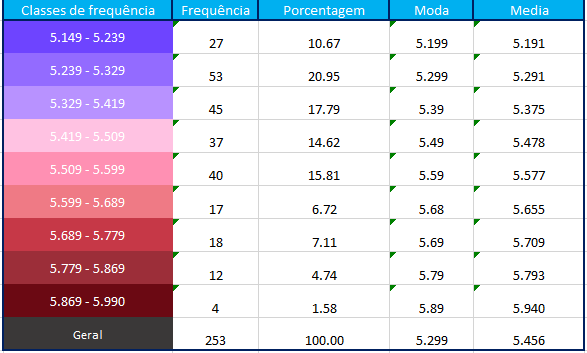
\includegraphics[width=\linewidth]{frequencias_pr.png}
    \caption{Tabela de frequências para os dados do Paraná.}
\end{figure}

\begin{figure}[H]
    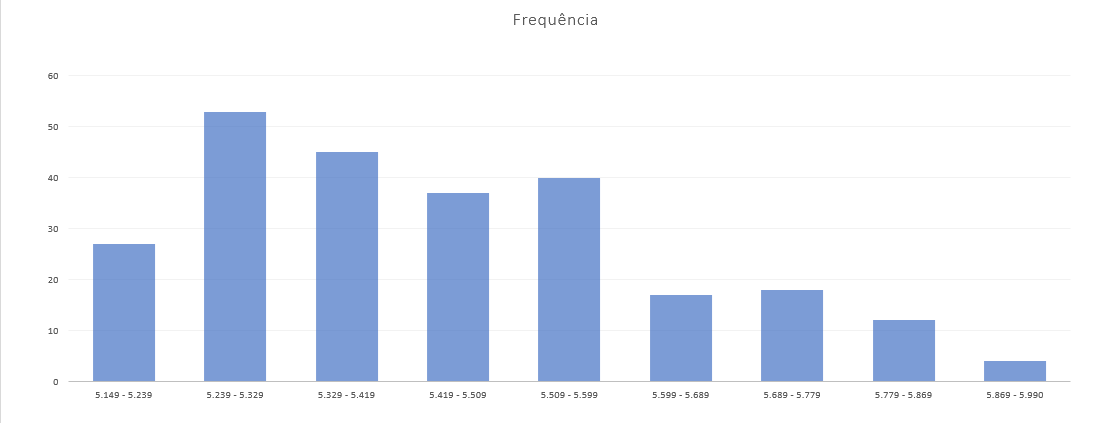
\includegraphics[width=\linewidth]{histograma_pr.png}
    \caption{Histograma das frequências para os dados do Paraná.}
\end{figure}

\subsection{Análise preliminar da coleta}

Após coletar os dados e aplicar o modelo empírico, foram geradas as tabelas de frequências e histogramas (Figuras de 1 a 4), com isso pudemos ver que o pico de frequencias em preços da gasolina comum se encontra em 5,720-5,800 para Minas Gerais e 5,239-5,329 para o Paraná. Ou seja, analisando apenas o dado de frequência de preços podemos notar que há uma maior incidência de preços altos em Minas Gerais do que no Paraná, o que provavalmente impacta fortemente no consumo final do produto.

\subsection{Análise descritiva dos dados}

Com os dados já organizados foi possível utilizar o software Excel e sua funcionalidade de aplicações de fórmulas para calcular moda, média e outros dados. O cálculo foi baseado em fórmulas presentes na bibliografia da disciplína e se encontram na próprias tabelas de frequências mostradas anteriormente.

\subsection{Análise exploratória dos dados}

Nessa última etapa, foi realizada uma comparação primeiramente entre estados, e em um segundo momento a análise foi feita em cima de uma separação de 3 bandeiras no estado do Paraná. Para isso, foram utilizados Box-Plots juntamente com a definição de quartis de Montgomery. Em nenhum dos casos foram encontrados outliers.

\begin{figure}[H]
    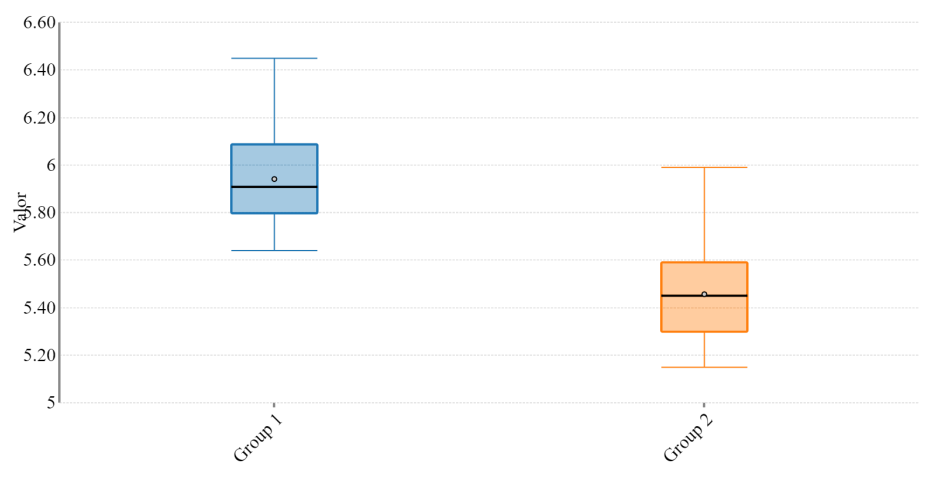
\includegraphics[width=\linewidth]{box_plot_pr.png}
    \caption{Box plot comparativo entre os estados.}
\end{figure}

\begin{figure}[H]
    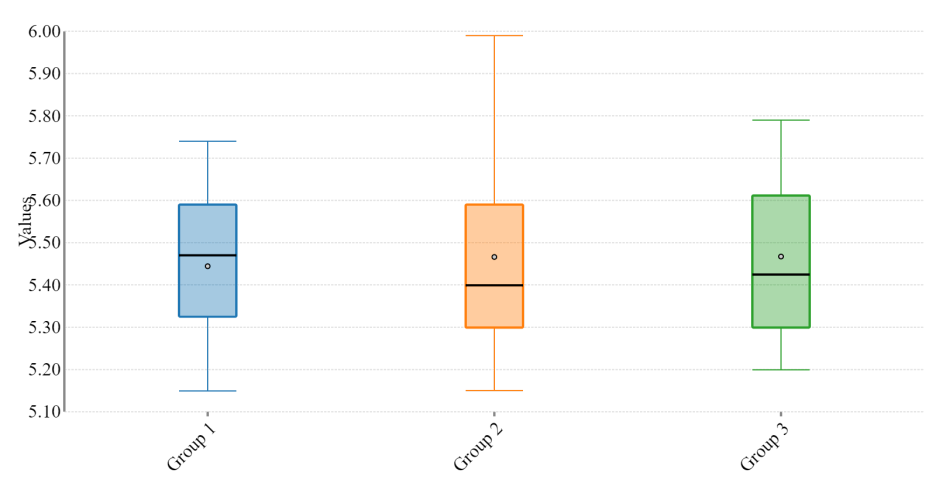
\includegraphics[width=\linewidth]{box_plot_bandeiras.png}
    \caption{Box plot comparativo entre bandeiras no Paraná.}
\end{figure}

\subsection{Conclusões}

Ao realizar uma análise comparativa entre os dois estados podemos perceber uma diferença considerável, onde o estado de Minas Gerais possui preços em média muito mais altos, o Box-Plot deixa isso ainda mais visível com a análise de quartis. Do ponto de vista do consumidor, além dos preços mais altos nos postos, é possível que preços de produtos comuns que sejam tranportados apenas dentro do estado também sejam encarecidos por essa alta no combustível.

A comparação entre as bandeiras nos mostra a primeira vista que as 3 possuem uma posição geral consistente, com suas medianas muito próximas. Além disso, os valores mínimos e os quartis também diferem em poucos centavos, nos dando a entender que existe uma boa equiparação de preços (ou possivelmente um cartel) entre as bandeiras.

Um dado acaba ficando discrepante no gráfico, o valor máximo da bandeira Ipiranga beira os 6 reais, aproximadamente 20 centavos acima dos valores máximos de suas concorrentes. De fato, ao voltarmos para nossa tabela de dados vemos que dentre todas as bandeiras, a Ipiranga possui os maiores valores máximos. Para o consumidor que tenha contato apenas com os postos onde o valor é alto, isso pode indicar que essa bandeira pratica preços mais altos do que as rivais, mas ao analisarmos a distribuição como um todo notamos que isso não é uma verdade.

\end{document}